\section*{Problema 18 del Capítulo 4}

\textbf{Enunciado:}

Trazar la gráfica de las funciones siguientes:

\begin{enumerate}
    \item $f(x) = \{x\}$, donde $\{x\}$ es la distancia de $x$ al entero más próximo.
    \item $f(x) = \{2x\}$.
    \item $f(x) = \{x\} + \frac{1}{2}\{2x\}$.
    \item $f(x) = \{4x\}$.
    \item $f(x) = \{x\} + \frac{1}{2}\{2x\} + \frac{1}{4}\{4x\}$.
\end{enumerate}

\textbf{Gráficas:}

\begin{figure}[h!]
    \centering
    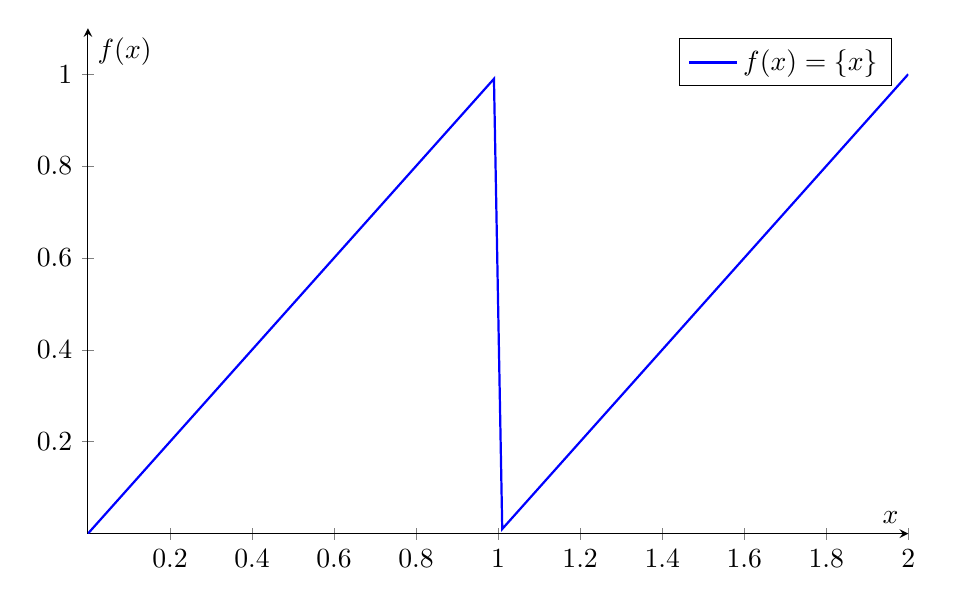
\begin{tikzpicture}
        \begin{axis}[
            axis lines = middle,
            xlabel = $x$,
            ylabel = {$f(x)$},
            ymin = 0, ymax = 1.1,
            xmin = 0, xmax = 2,
            width=12cm,
            height=8cm
        ]
        % Gráfica de f(x) = {x}
        \addplot[domain=0:2, samples=100, blue, thick] {x - floor(x)};
        \addlegendentry{$f(x) = \{x\}$}
        \end{axis}
    \end{tikzpicture}
    \caption{Gráfica de $f(x) = \{x\}$.}
    \label{fig:fx_modulo}
\end{figure}

\begin{figure}[h!]
    \centering
    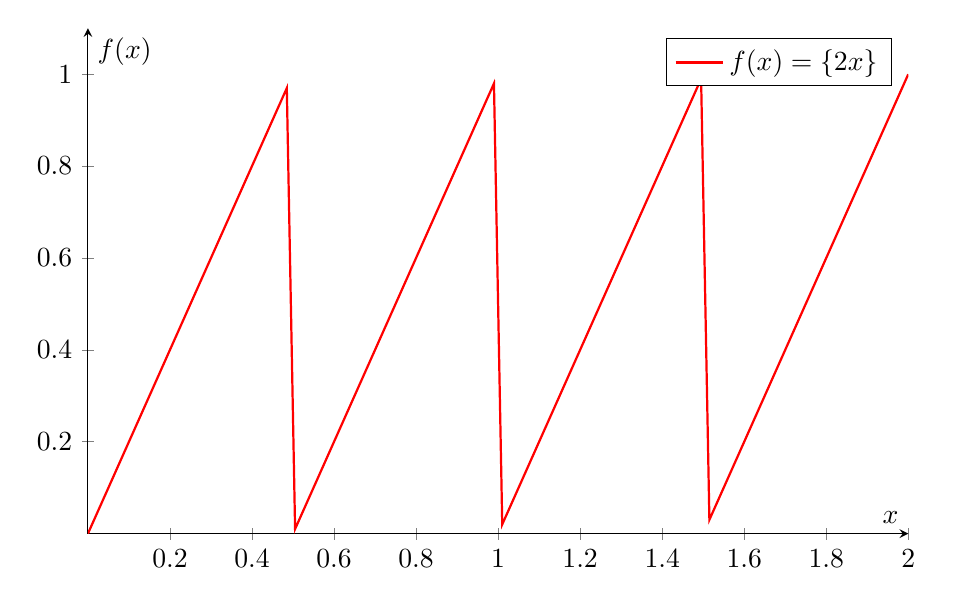
\begin{tikzpicture}
        \begin{axis}[
            axis lines = middle,
            xlabel = $x$,
            ylabel = {$f(x)$},
            ymin = 0, ymax = 1.1,
            xmin = 0, xmax = 2,
            width=12cm,
            height=8cm
        ]
        % Gráfica de f(x) = {2x}
        \addplot[domain=0:2, samples=100, red, thick] {2*x - floor(2*x)};
        \addlegendentry{$f(x) = \{2x\}$}
        \end{axis}
    \end{tikzpicture}
    \caption{Gráfica de $f(x) = \{2x\}$.}
    \label{fig:fx_2x}
\end{figure}

\begin{figure}[h!]
    \centering
    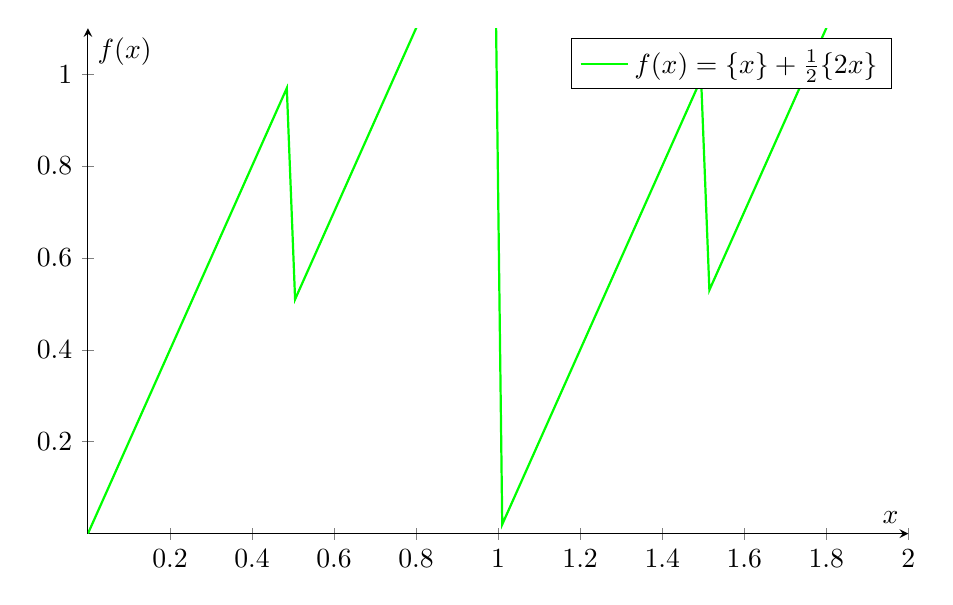
\begin{tikzpicture}
        \begin{axis}[
            axis lines = middle,
            xlabel = $x$,
            ylabel = {$f(x)$},
            ymin = 0, ymax = 1.1,
            xmin = 0, xmax = 2,
            width=12cm,
            height=8cm
        ]
        % Gráfica de f(x) = {x} + 1/2{2x}
        \addplot[domain=0:2, samples=100, green, thick] {x - floor(x) + 0.5*(2*x - floor(2*x))};
        \addlegendentry{$f(x) = \{x\} + \frac{1}{2}\{2x\}$}
        \end{axis}
    \end{tikzpicture}
    \caption{Gráfica de $f(x) = \{x\} + \frac{1}{2}\{2x\}$.}
    \label{fig:fx_combined}
\end{figure}

\begin{figure}[h!]
    \centering
    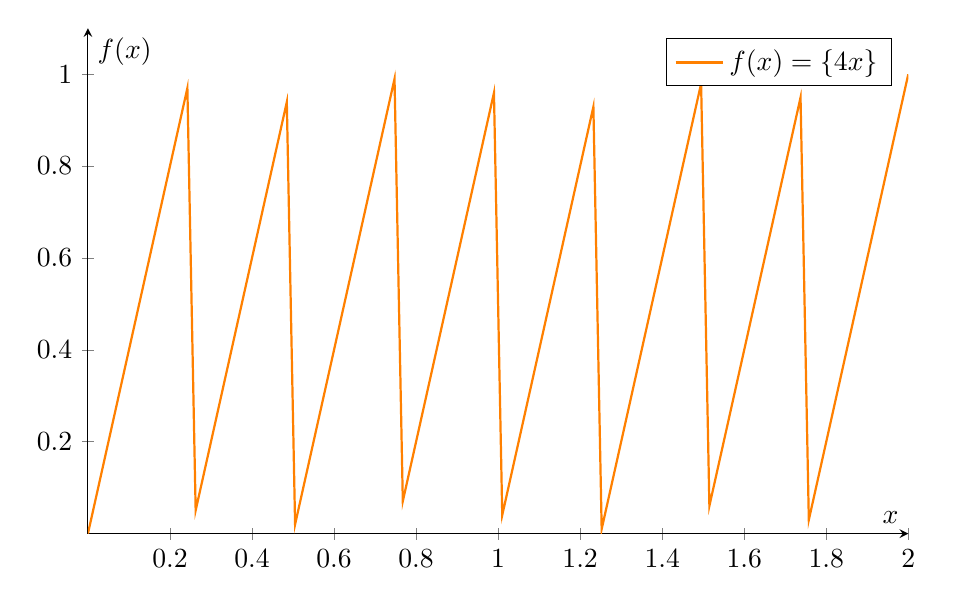
\begin{tikzpicture}
        \begin{axis}[
            axis lines = middle,
            xlabel = $x$,
            ylabel = {$f(x)$},
            ymin = 0, ymax = 1.1,
            xmin = 0, xmax = 2,
            width=12cm,
            height=8cm
        ]
        % Gráfica de f(x) = {4x}
        \addplot[domain=0:2, samples=100, orange, thick] {4*x - floor(4*x)};
        \addlegendentry{$f(x) = \{4x\}$}
        \end{axis}
    \end{tikzpicture}
    \caption{Gráfica de $f(x) = \{4x\}$.}
    \label{fig:fx_4x}
\end{figure}

\begin{figure}[h!]
    \centering
    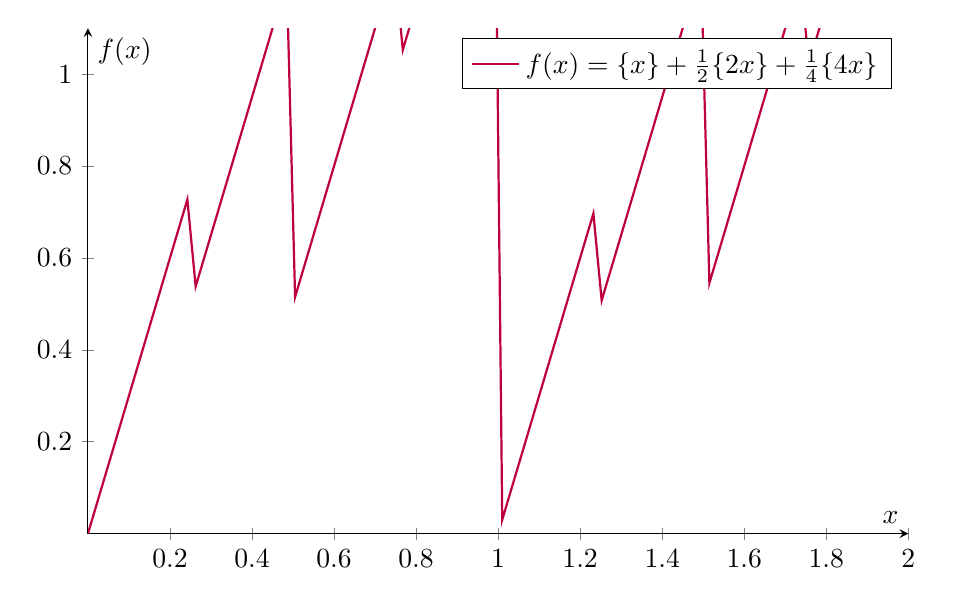
\begin{tikzpicture}
        \begin{axis}[
            axis lines = middle,
            xlabel = $x$,
            ylabel = {$f(x)$},
            ymin = 0, ymax = 1.1,
            xmin = 0, xmax = 2,
            width=12cm,
            height=8cm
        ]
        % Gráfica de f(x) = {x} + 1/2{2x} + 1/4{4x}
        \addplot[domain=0:2, samples=100, purple, thick] {x - floor(x) + 0.5*(2*x - floor(2*x)) + 0.25*(4*x - floor(4*x))};
        \addlegendentry{$f(x) = \{x\} + \frac{1}{2}\{2x\} + \frac{1}{4}\{4x\}$}
        \end{axis}
    \end{tikzpicture}
    \caption{Gráfica de $f(x) = \{x\} + \frac{1}{2}\{2x\} + \frac{1}{4}\{4x\}$.}
    \label{fig:fx_combined_2}
\end{figure}